\documentclass{article}
\usepackage{multicol}
\usepackage{graphicx}
\usepackage[top=1.03in, bottom=0.51in, left=0.93in, right=0.92in]{geometry}

\usepackage{color}
\usepackage{url}
\usepackage{hyperref}
\definecolor{linkcolour}{rgb}{0,0.2,0.6} 
\hypersetup{colorlinks,breaklinks,urlcolor=linkcolour, linkcolor=linkcolour}  
\usepackage{pdfpages}

%wrapfig
\usepackage{wrapfig}
\usepackage{lipsum}  % generates filler text

\renewcommand{\familydefault}{\sfdefault} 

\renewcommand{\labelenumi}{\Roman{enumi}. }

\begin{document}
\definecolor{orange}{rgb}{0.9648,0.4960,0}

\begin{figure}[ht]
\begin{minipage}[t]{0.40\linewidth}
\centering
\raisebox{-\height}{
\includegraphics[width=2in]{UT-logo2.png}}

\label{fig:figure1}
\end{minipage}
\hspace{0.5cm}
\begin{minipage}[t]{0.5\linewidth}
\centering 
\vskip 0.2cm
\textcolor{orange}{\huge \bf CASE STUDY}
\vskip 0.2cm 
{\Large \bf Modeling and Simulation}
\vskip 0.2cm 
{\Large \bf Dr. Xueping Li }

\end{minipage}
\end{figure}
{\bf
\begin{tabular}{ll}
%Course Section:	& IE 526 \\
\textcolor{orange}{------------------------------------------------------------------------------------------------------------------------------}
\end{tabular}
}

%%\vskip 0.3in

\begin{center}
{\textcolor{orange}{ \bf Case Study: Network-based Models \& 3D Animation}}
\end{center}
\vskip 0.2in

%\begin{enumerate}

%\item 

\textcolor{orange}{\bf Goal::} \textit{To learn the following methods/techniques:}\\
\begin{itemize}

\item How to define a connected network
\item Use ``MoveTo, Seize, Delay, Release, Resource Attach/Detach, Resource Pool, Resource Task Start/End'' modules 
\item 3D animation, ``3D window, light, camera''
\item Source arrival: rate schedule, arrival schedule
\item Update ResourcePool capacity pr
\end{itemize}


\vskip 0.3in

\textcolor{orange}{\bf Problem Statement:}  In this section of the tutorial we will build a model of a typical ophthalmology unit. Patients arrive to the department to undergo the ophthalmoscopy procedure. They are held in the waiting room and wait for�ophthalmologists to come and make an examination. The procedure is held in the procedure room. When a doctor arrives,�patient moves to empty procedure room escorted by the doctor. The procedure is performed using an ophthalmoscope. Ophthalmoscopes are stored in the storage room and are taken by doctors just before the procedure begins. Following the procedure, the doctor transports the ophthalmoscope back to the storage room and returns to the staffroom, and the patient leaves the ophthalmology department.

\begin{figure}[htbp]
\begin{center}
	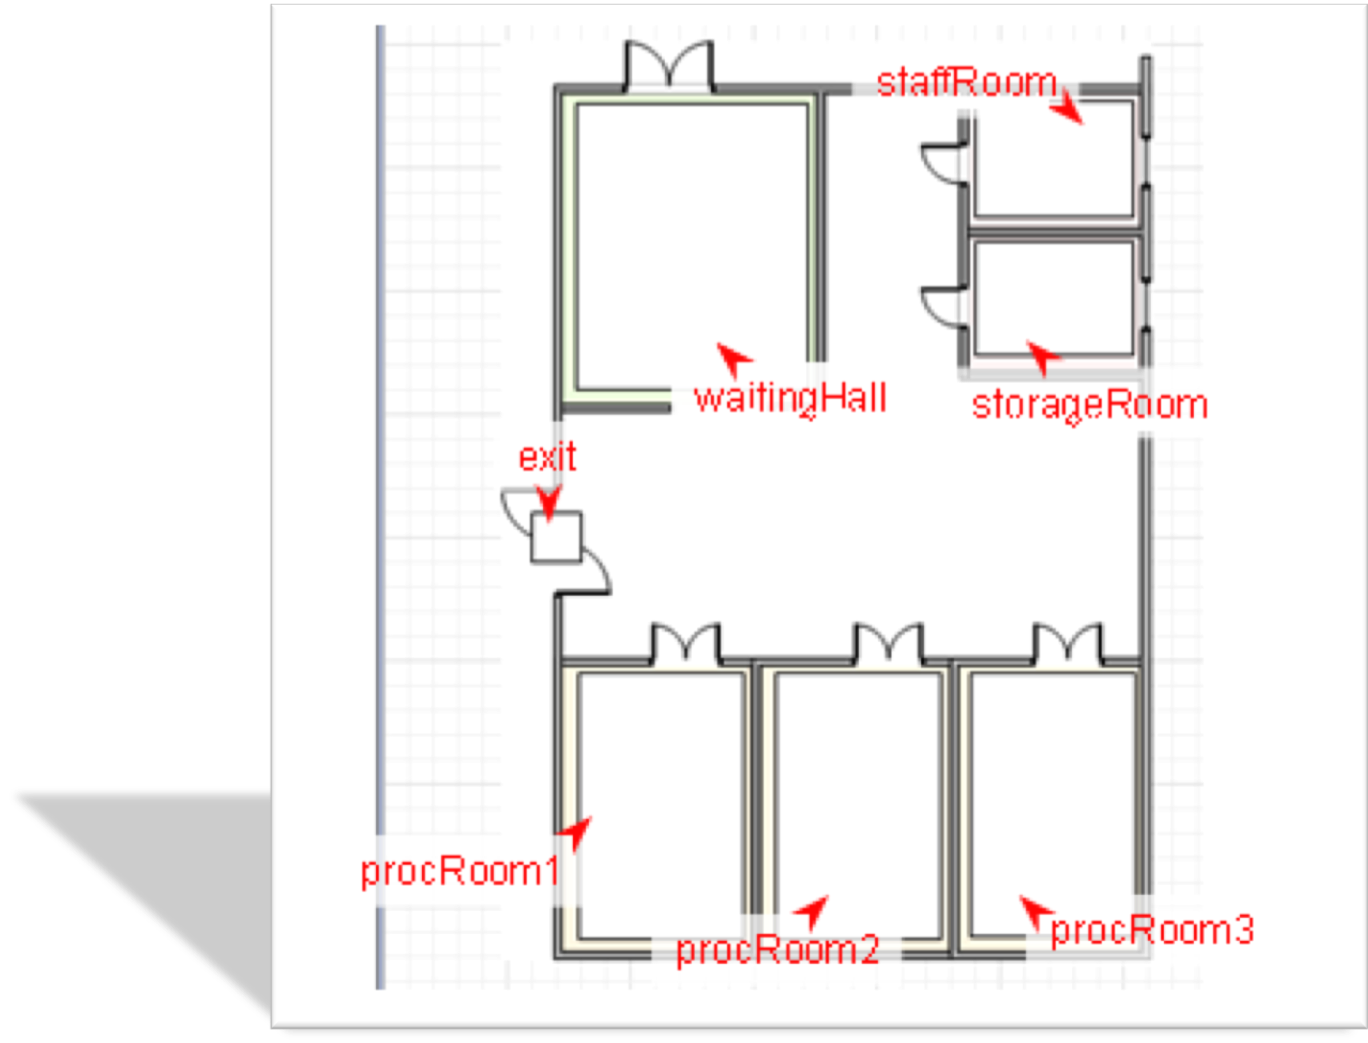
\includegraphics [width=0.50\textwidth] {network_eyedoc.png}
\caption{``Layout System'':  Eye Clinic}
\label{fig:sp}
\end{center}
\end{figure}

\end{document}

